\documentclass{llncs}
\usepackage{amsmath}
\usepackage{amsfonts}
\usepackage{amssymb}
\usepackage{algpseudocode}
\usepackage{algorithm}
\usepackage{subfig}
\usepackage{xcolor}
\usepackage{graphicx}
\usepackage{url}
\newcommand{\X}{{\bf X}}
\newcommand{\x}{{\bf x}}
\newcommand{\p}{{\bf p}}
\newcommand{\rr}{{\bf r}}
\newcommand{\I}{\image{I}}
\newcommand{\V}{{\bf V}}
\newcommand{\vv}{{\bf v}}
\newcommand{\h}{{\bf H}}
% {\Large \bf  Eigenanatomy: A sparse anatomical decomposition method for a ``cluster then threshold'' approach to morphometry} \\
\title{Fusing functional signals by sparse canonical correlation analysis improves network reproducibility}
% \author{Anon}
% \institute{Penn Image Computing and Science Laboratory}
\begin{document}
\maketitle
\begin{abstract}
We contribute a novel multivariate strategy for computing brain network structure from arterial spin labeling (ASL) MRI.  Our method, X, fuses and correlates multiple functional signals by employing an interpretable dimensionality reduction method, sparse canonical correlation analysis (SCCA).  There are two key aspects of this contribution.  First, we show how SCCA may be used to compute a multivariate correlation between different regions of interest (ROI).  In contrast to averaging signal over the ROI, this approach exploits the full information within the ROIs.  Second, we show how SCCA may simultaneoulsy exploit both the ASL-BOLD and ASL-based cerebral blood flow (CBF) time series to produce network measurements.  Our approach to fusing multiple time signals in network studies improves reproducibility over standard approaches while retaining the interpretability afforded by the classic ROI seed-based methods.  We show experimentally in test-retest data that our sparse CCA method extracts biologically plausible and stable network structures from ASL.  We compare the ROI approach to the CCA approach while using CBF measurements alone.  We then compare these results to the joint BOLD-CBF networks in a reproducibility study and in a study of network structure in traumatic brain injury (TBI).  In TBI, standard region-based approaches may fail due to local injury which makes averaging over a full ROI less meaningful.  We detail the algorithm and show experimental evidence of its efficacy in a clinically relevant TBI population.  Our results show th
\end{abstract}

\section{Introduction}
Functional MRI (fMRI) is capable of measuring subject-specific and long-range correlations in brain activity (i.e. networks) as measured by changes in a direct or indirect time-series measurement of cerebral blood flow (CBF).  EPI-BOLD is the standard protocol for studying network structure \cite{Bullmore2009}.  A second approach, arterial spin labeling (ASL) MRI, more directly measures CBF by tagging arterial blood and tracking changes in magnetization over time. ASL provides a quantitative measure of blood flow, which is believe to be more directly related to neuronal activity than the measure provided by EPI-BOLD \cite{Wong1997}.  ASL-based CBF time series are are less frequently studied in network analysis in part due to the relatively recent availability of the CASL, pCASL or PASL MR sequences.  One advantage of ASL is greater signal stability and reproducibility when compared to EPI-BOLD especially over the range of resting state frequencies \cite{Aguirre2002}.  Additionally, the ASL acquisition contains images that exhibit BOLD contrast (ASL-BOLD) \cite{Wong1997}, although the temporal resolution of ASL is lower than EPI-BOLD, resting state fluctuations are thought to reside well within the range of frequencies that may be captured by ASL ( 0 Hz to 0.1 Hz ) \cite{Cordes2001}.  Thus, ASL may prove to be a valuable quantitative technique for measuring large-scale human brain networks.

While EPI-BOLD has been used extensively to examine functional brain connectivity in large-scale brain networks, only a small number of studies have examined functional connectivity in ASL \cite{Chuang2008,Zou2009}. Additionally, two studies have compared ASL-connectivity and BOLD connectivity meaured with either EPI-BOLD \cite{Li2012}, or ASL-BOLD \cite{Viviani2011}.  To our knowledge no previous work has combined the CBF and BOLD components of the ASL signal to obtain a functional connectivity measure that exploits the full information provided by this modality. The scarcity of related work may be due, in part, to the fact that most ASL sequences collect relatively fewer time frames (impacting the stability of correlations) in a given amount of scan time as well as the lack of off-the-shelf methodology for computing ASL networks.  A second reason may be that ASL is used primarily for computing CBF measurements in a manner similar to PET \cite{Chen2008}.  While ASL has been used to examine mean CBF in TBI \cite{Hart2013}, there is also little to no work employing ASL-connectivity in TBI.   This population is difficult due to the heterogeneity of injury and the likely presence of cortical injury which may make standard analysis approaches difficult to justify. 

In this work, we contribute a new multivariate method for ASL-based network analysis.  We improve upon existing approaches in two ways.  First, we extend standard region-based methods with a sparse dimensionality reduction method that optimally correlates two ROIs.  This is achieved by formulating the correlation between ROIs as a sparse selection optimization algorithm that finds non-uniformly weighted sub-ROIs that are most related.  Second, we show how this method may jointly find these sub-ROIs by using both ASL-BOLD and CBF time series signal.  Both of these advances relax some of the assumptions of standard region-based approaches while retaining the interpretability afforded by these classic approaches.  

In short, our contributions are: 
\begin{enumerate}
\item We detail a new multivariate network analysis method.
\item We show how it may be used to fuse simultaneous time series measurements from multiple signal sources to estimate correlation matrices.
\item We evaluate these approaches in terms of reproducibility and applicability to studying TBI. 
\end{enumerate}
The method is freely available in a public open source toolkit \cite{anon}.


\section{Methods}
Canonical correlation analysis (CCA) as originally proposed as a method for elucidating the relationship between two set of measurements taken across a population \cite{Hotelling1936} and is thus a well-suited basis for the examination of multi-variate neuroimaging data.  We compare a novel CCA based method to the classic region averging approach. Here, we denote the matrices that describe the ASL-BOLD or ASL-CBF time series within a whole-brain ROI as $X$ and $Y$ respectively.  Additionally, for a given set of anatomical ROIs for which there are $L$ regions, we denote the ASL-BOLD sub-matrix extracted from ROI$^i$ as $X^i$.  Then $Y^i$ will contain that same ROI's ASL-CBF measurements. The classic region-based analysis will compute $x^i = 1/n \sum_k x^i_k$ which denotes averaging the $x^i_k$ columns of $X^i$ and similarly for $y^i$.  From these region-averaged time-signals, a correlation matrix, $\mathcal{R}$, of size $L \times L$ is calculated, where $\mathcal{R}(i,j)=Corr(x^i,x^j)$ with $Corr$ denoting the Pearson's correlation. This correlation matix then serves as the basis for graph-based analysis. To serve as a basis for later comparison, A correlation matrix was also computed from concatenated averaged ASL-BOLD and ASL-CBF time series data.

\subsection{Fusing functional signals via SCCA}
Canonical correlation analysis (CCA) generalizes the approach described above \cite{Hotelling1936}.  CCA introduces new unknown vectors, $u^i$ and $u^j$, that act as weighted averages of $x^i, x^j$.  CCA will optimize:
\begin{equation}
\underset{u^i,u^j}{\operatorname{arg\,max}} \quad~ Corr(~u^i~X^i,~u^j~X^j~) 
\end{equation}
This formulation allows for the inclusion of the full time signal in all voxels in an ROI and is ``nice'' in that it can be solved by singular value decomposition if the number of samples is larger than the minimum number of columns in $X^i$ or $X^j$. Sparse CCA extends CCA with additional constraints that allow the problem to be solved even when the input matrices are ``fat'' i.e. the number of columns far exceeds the number of rows, as is typically the case in fuctional MRI data.  The SCCA formulation optimizes: 
\begin{gather*}
\underset{u^i,u^j}{\operatorname{arg\,max}} \quad~ ~~u^i~(X^i)^T ~X^j~u^j~\\ \notag \text{subject to} \\ \notag
\sum_i \|u^i\|_1 \leq s, ~~ u^i \ge 0,~~ \sum_i \|u^j\|_1 \leq t, ~~ u^j \ge 0 , ~~\| A X_i \| = \| B Y_i \| = 1,
\end{gather*}
where $s, t$ determine sparseness.  Due to the non-linear (even np-hard) nature of this problem, optimizing for a single canonical variate, $u_i$, involves a nonlinear gradient descent on the objective function above.  This is one disadvantage of these methods.  However, one gains robustness and the ability to exploit the full information of the input data. An addtional advantage is that the formulation shown above may be easily exteneded to incorporate both ASL-CBF and ASL-BOLD data for simultaneous analysis. For a given ROI, $\X^i$ is an $n \times p$ (rows by columns) matrix where $n$ is the number of acquired time points and $p$ is the number of voxels in ROI$^i$. Since both ASL-CBF and ASL-BOLD derive from the same acquisition, $X^i$ and $Y^i$ will always have the same dimensions. To examine both metrics simultaneously we can column-append the two matrices: $Z^i = \left[ \left[X^i\right] \left[Y^i\right] \right]$ resulting in a $n \times 2p$ matrix. For clarity, $\X$ will be used in further equations with the knowledge that it could be replaced with $Y$ or $Z$ with no resulting changes to the algorithm.

%The class of methods encompassing non-negative matrix factorization
%(NMF) \cite{Lee1999,sparseNMF_hoyer,sparseNMF_kim,sparseNMF_heiler},
%sparse principal components analysis (SPCA)
%\cite{sparsePCA_zou,sparsePCA_jordan,sparsePCA_journee,sparsePCA_witten,Gandy2010,Lee2011}
%and singular value decomposition \cite{Sill2011,Lee2010b,Yeung2002}
%form the basis for the approach proposed here.
 
More generally, $\X$ is an $n \times p$ matrix where each row represents observations at a given time and each column is a time-signal within a voxel. We then define a set of canonical variates $\{ v_i,...,v_n\}$ where each $v_i$ is ordered such that each variate from $v_1$ to $v_n$ provides a decreasing contribution to the variance of $X$. Here, we want to enforce sparseness, meaning that some entries in $v_i$ will be zero. The classic singular value decomposition (SVD) may be used to reduce the dimensionality of this data by decomposing the dataset into the eigenvectors of $C_p = \X^T\X$ and $C_n = \X\X^T$ (the right and left singular vectors, respectively).  The relationship between a $C_p$ and a $C_n$ eigenvector is given by $\X \vv^p = \vv^n$ and $\X^T \vv^n = \vv^p$.  The $n$ eigenvectors from $C_p$ and $C_n$ may be used to reconstruct the matrix $\X$ by $\sum_i \vv^n_i \otimes \vv^p_i \lambda_i $ where the $\lambda_i$ denotes the $i^{th}$ eigenvalue and $\otimes$ the outer product.

%as vectors $\{x_1,...,x_n\}$ with each vector $x_i$ containing $p$ entries.  irst, we denote each eigenanatomy component (a pseudo-eigenvector) as
%${\vv}_i$ where $i$ is ordered such that each eigenanatomy from
%${\vv}_1$ to ${\vv}_m$ provides a decreasing contribution to the
%variance of matrix $\X$.  We define eigenanatomy pseudo-eigenvectors as {\em
 % sparse}.  Sparseness means that some entries in ${\vv}_j$ will be zero.
 
Our goal is to approximate the matrix $\X$ with its right and left singular vectors but where the right singular vector is {\em sparse}.  We might, then, minimize:
\begin{eqnarray}
\label{eq:recon}
\| \X  -  \sum_i \vv^n_i \otimes \vv^{sp}_i \lambda_i  \|^2
\end{eqnarray}
where the $\vv^{sp}_i$ denotes the $i^{th}$ {\em sparse} right singular vector.  However, it is known that the minimizer, here, is exactly $\X^T \vv^n$ ( if we relax sparseness constraints ).  Using the fact that $\X \vv^p = \vv^n$ and $\X^T \vv^n = \vv^p$,  we therefore reformulate the objective in a slightly simpler form and seek:
\begin{eqnarray}
\label{eq:basic}
\underset{\vv^{sp}_i}{\operatorname{arg\,min}}~~\|  \X \vv^{sp}_i - \vv_i^n \|^2 . 
\end{eqnarray}
This optimization problem is quadratic without sparseness constraints and easily solved by conjugate gradient through the normal equations $\| \X^T\X \vv^{sp}_i - \X^T\vv_i^n \|^2$.

Now, note that the vector $\X^T\vv_i^n=\vv_i^p$ might have both positive and negative values.  As with non-negative matrix factorization, we seek a decomposition that is unsigned.   However, an optimal solution that minimizes $\|  \X \vv^{sp}_i - \vv_i^n \|^2$ will need to model both signs.  We therefore make a second adjustment to our objective by modeling the positive and negative components of $\vv_i^p$ separately.

Each eigenvector may be written in an expanded form via the use of indicator functions which are diagonal matrices with binary entries.  For instance, if $\vv$ contains entries $[~-2,~-1,~0,~1,~2~]$, then the positive indicator function is $I^+=[~0,~0,~0,~1,~1~]$ and the negative indicator function is $I^-=[~1,~1,~0,~0,~0~]$.  $\vv$ may then be expressed as $\vv = I^+\vv + I^- \vv = \vv^+ + \vv^-$.  We use these indicator functions to separate the positive and negative components of our objective such that the optimization in equation~\ref{eq:basic} becomes,
\begin{equation}
\label{eq:basic2}
\underset{\vv^{sp+}_i~,~\vv^{sp-}_i}{\operatorname{arg\,min}}~~\|  \X^T\X \vv^{sp+}_i - \vv_i^{p+} \|^2 + \|  \X^T\X \vv^{sp-}_i - \vv_i^{p-} \|^2  
\end{equation}
This minimization problem forms the basis for our approach to identify correlated activity between ROIs.

As noted above, we seek sparse and interpretable solutions.  We define a sparse vector as one which minimizes a $l_0$ or $l_1$ penalty term i.e. has either a user-specified number of non-zero entries ($l_0$) or absolute sum ($l_1$).  Although the $l_1$ penalty has advantages \cite{sparsePCA_zou},  we use the $l_0$ penalty because it specifies the fraction of the vector that is allowed to be non-zero.  The sparseness restriction is therefore easily interpreted by users of the eigenanatomy method.  The eigenanatomy objective seeks to identify sparse functions $\vv_i^{sp+}$ and $\vv_i^{sp-}$ that closely approximate the eigenvectors in $n$-space, i.e. $\vv^i_n=\X \vv_i^p$.  The objective function is then:
\begin{eqnarray}
\label{eq:eigenanatomy}
\underset{\vv_i}{\operatorname{arg\,min}}~~\sum^n_{i=1}~~\|~C_p \vv_i^{sp+} - \vv_i^{p+} ~\|^2 + \|~C_p \vv_i^{sp-} - \vv_i^{p-} ~\|^2 \\ 
\text{subject to:}~~~  \| \vv_i^{sp+} \|_0 =  \| \vv_i^{sp-} \|_0 = \gamma,\notag
\end{eqnarray}

where $\gamma$ defines the desired level of sparseness for each eigenanatomy vector.  
Eigenanatomy therefore produces $2*n$ sparse pseudo-eigenvectors whose product with $\X$ may be used a predictors in standard linear regression.  Importantly, because these vectors are unsigned, they may be interpreted as {\em weighted averages of the input data.}  

Sparseness can be enforced by a soft-thresholding algorithm as in \cite{sparsePCA_zou,sparsePCA_witten}.  We denote this function as $S( \vv , \gamma)$ and (in an {\em adhoc} manner) allow it to also reject isolated voxels of the eigenanatomy vector that are non-contiguous (i.e. we provide a cluster threshold as in VBM).  Minimization problems involving the $l_0$ penalty are $np$-hard.  However, the relaxed form of this objective function (i.e. without the sparseness constraint) is purely quadratic and can easily be solved by a conjugate gradient method.  Thus, we propose a new sparse, nonlinear conjugate gradient (SNLCG) method as a minimization procedure for the eigenanatomy objective function to deal with the nonlinearities induced by the $S$ function and $l_0$ constraint.  Such methods are efficient and reliable for sparse estimation methods \cite{marjanovic2010}.  The additional advantage of SNLCG is that its solutions approach the quadratic minimum as sparseness constraints are relaxed.  We detail the minimization algorithms for the eigenanatomy objective function (equation~\ref{eq:eigenanatomy}) in algorithms~\ref{alg:eigenanatomy} and~\ref{alg:snlcg}.  The algorithms are also available in an open-source {\bf R} package for free use. 


\section{Results}

\subsection{Evaluating reliabity via test-retest data}
\noindent{\bf Neuroimaging data:}The cohort consists of 12 healthy young adults ( age info ) participants (N female). For each subject, data was acquired at three time points. Two of these time points were acquired on the same day, in separate scanning sessions, while the third was acquired one week away from the same-day data.  For each time point High resolution T1-weighted anatomic images were obtained using 3D MPRAGE imaging sequence and the following acquisition parameters: TR = 1620 ms, TI = 950 ms, TE = 3 ms, flip angle = 15 degrees, 160 contiguous slices of 1.0 mm thickness, FOV = 192 $\times$ 256 mm$^2$, matrix = 192 $\times$ 256, 1NEX with a scan time of 6 min. The resulting voxel size was 1 mm.  Additionally, pulsed ASL (PASL) images were aquired with 80 alternating tag/control images and 2 M0 images all with 14 contiguous slice of 7.5mm thickness, FOV = 220 $\times$ 220mm$^2$, matrix = 64 $\times$ 64. Additional acquisition parameters: TI1 = 700ms, TI2 = 1700ms.

\noindent{\bf Image processing:} The set of T1 images from each subjects first time points was used to construct a template using ANTs \cite{Avants2011}. This template was brain masked and labeled with the AAL dataset \cite{Tzourio-Mazoyer2002}. Additionally, the a three-tissue segmentation of the template allowed the labels to be partially masked so only cortex and deep gray structures were labeled. For each time point, the T1 image was registered to the template image. Additionally, registration was used to find an intra-subject mapping between the T1 image and the M0 image that is acquired as a reference for the PASL acquisition. These transforms were composed to map the cortical labels into ASL native space for each time point. For PASL images, the M0 image served as a reference for motion-correction of all time-point volumes. Sinc interpolation was used to estimate the full time-series for both the control and tag data. The difference between control and tag was used along with relevant acquisition parameters to calculate the ASL-CBF over time, while the average of the two signals was calculated for ASL-BOLD \cite{Wong1997}. 

To examine consistency, connectivity matrices are calculated for each time point using the classic region-averaged approach and the SCCA method on: ASL-CBF, ASL-BOLD, and combined ASL-CBF and ASL-BOLD. Graph correlation \cite{vanWijk2010} is used for the comparison of connectivity matrices in order to examine reproducibility between images acquired on the same day, and image acquired one week apart as illustrated in figure \ref{fig:testretest}.

\begin{figure}[tb]
\begin{center}
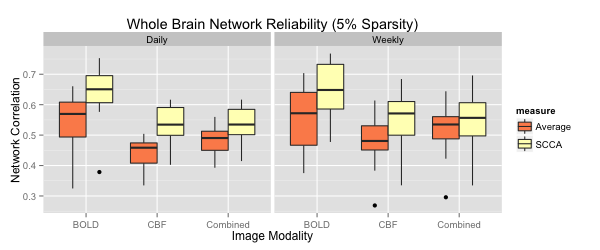
\includegraphics[width=0.75\linewidth]{retest.png} 
\caption{For each metric, using both region averaging (orange) and SCCA (yellow), connectivity matrices calculated from ASL data acquired in separate acquisitions in the same day and for data acquired one week apart. Network correlations were then calculated to examine reliability for the daily (left) and weekly (left) data for each subject. Here we illustrate results using a sparsity value of 0.05. A range of sparsity values up to 0.25 examined and these higher values did not produce significantly different results.}
\label{fig:testretest}
\end{center}
\end{figure}

\subsection{Cross-sectional examination of brain connectivity in TBI}
\noindent{\bf Neuroimaging data:} Our cohort consists of 41 participants, including 22 patients with TBI (9 females), and 18 controls (9 females). No significant difference exist between age or education in the patient or control groups.  The same image T1 acquisition as decribed above was used for these subjects.

\noindent{\bf Image processing:} Processing for this data is identical to that for the test-retest data described above. The pulsed ASL (PASL) images were aquired with 160 alternating tag/control images and 2 M0 images all with 14 contiguous slice of 7.5mm thickness, FOV = 220 $\times$ 220mm$^2$, matrix = 64 $\times$ 64. Additional acquisition parameters: TI1 = 700ms, TI2 = 1900ms.

To identify potential effects of TBI, CBF-BOLD connectivity matrices were calculated for all subjects. In particular, the default mode network is of interest as this network has been shown to be affected by TBI \cite{} and is relevant here as the data was acquired during the resting state. Here we used the following labeled regions for the default mode network: posterior cingulate gyrus, hippocampus, frontal medial orbital cortex, and the angular gyrus. Each subject was categorized as either: No injury, less than one year since injury or more than one year since injury. For each metric of interest, connectivity values for intra-hemispheric connections in each hemisphere were extrated and $R$ was used examine the influence of diagnosis (TBI or control) on connectivity values using (in $R$ syntax):
\begin{equation}
Conn \sim 1 + Diagnosis + Age + Gender + YearsEducation + InjuryTime
\end{equation}
All p-values for Diagnosis were FDR corrected and connections with p<0.1 were reported. The region-averaging approach did not result in any reported connectivity differences, nor were any results reported for ASL-BOLD alone. Connecitivity measured using SCCA on the ASL-CBF and the combined data both reported connectivity differences in the right hemisphere between the posterior cingulate gyrus and both the hippocampus and angular gyrus.
 
\begin{figure}[tb]
\begin{center}
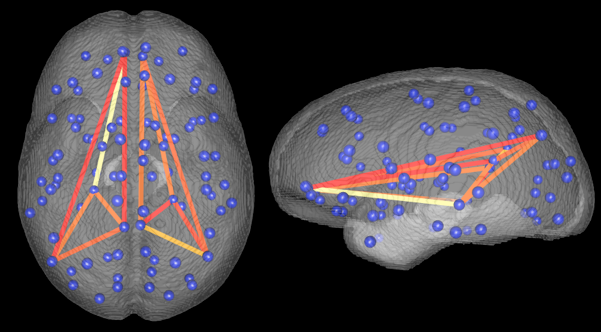
\includegraphics[width=0.5\linewidth]{dfm.png} 
\caption{This is a temporary placeholder image}
\label{fig:dfm}
\end{center}
\end{figure}

\section{Conclusion}
We detailed how SCCA may be used to fuse the ASL-CBF and ASL-BOLD signals to exploit both the multi-variate signal provided by ASL as well as the full information provided within each anatomical region. We demonstarted that the SCCA method provides a more repeatable measure of network connectivity than the classic region-averaged approach. An addtional examination of TBI suggested that the SCCA method provides a measure of connectivity that is more sensitive to disruptions in the default mode network.  Future work will include exploring how additional modalities, such as standard BOLD fMRI, may be incorporated into the framework described here.

\bibliographystyle{splncs}
\bibliography{refs}

\end{document}
